% =============================================================================
%  APÊNDICE F: GUIA DE REFERÊNCIA RÁPIDA E LINHA DO TEMPO
%  Cheatsheet CLI, arquitetura, scanners, SPECs, evolução e glossário
% =============================================================================
\chapter{Guia de Referência Rápida e Linha do Tempo}
\label{ap:cheatsheet}

% =============================================================================
%  SEÇÃO 1: CHEATSHEET DE COMANDOS OPENCODE CLI
% =============================================================================
\section*{Comandos OpenCode CLI}

\begin{table}[htb]
\centering
\caption{Comandos principais do \opencodeeco{}}
\label{tab:cheatsheet-comandos}
\small
    \resizebox{\textwidth}{!}{
\begin{tabular}{lll}
\toprule
\textbf{Comando} & \textbf{Descrição} & \textbf{Exemplo} \\
\midrule
\codigo{/evolve} & Ciclo evolutivo completo & \codigo{/evolve --full} \\
\codigo{/evolve --scan-only} & Apenas scanners, sem roadmap & \codigo{/evolve --scan-only} \\
\codigo{/plan} & Planejamento de escrita & \codigo{/plan ``artigo sobre IA''} \\
\codigo{/artigo} & Pipeline completo de artigo Qualis A1 & \codigo{/artigo --tema ``educação''} \\
\codigo{/reversa} & Engenharia reversa de projeto & \codigo{/reversa --projeto ./src} \\
\codigo{/scan noological} & Scanner noológico & \codigo{/scan noological --dominio computacao} \\
\codigo{/scan teleological} & Scanner teleológico & \codigo{/scan teleological --objetivo causal} \\
\codigo{/quantum} & Pipeline quantum nexus PhD & \codigo{/quantum --ham10000} \\
\codigo{/auto} & Modo automático com todos MCPs & \codigo{/auto} \\
\codigo{/marceloclaro} & Orquestrador central & \codigo{/marceloclaro ``analise ecossistema''} \\
\bottomrule
\end{tabular}
    }
\end{table}

\begin{table}[htb]
\centering
\caption{Flags e atalhos dos comandos}
\label{tab:cheatsheet-flags}
\small
    \resizebox{\textwidth}{!}{
\begin{tabular}{lll}
\toprule
\textbf{Comando} & \textbf{Flag} & \textbf{Efeito} \\
\midrule
\codigo{/evolve} & \codigo{--full} & Executa ciclo completo (scanners + roadmap) \\
\codigo{/evolve} & \codigo{--scan-only} & Executa apenas scanners, sem gerar roadmap \\
\codigo{/evolve} & \codigo{--dry-run} & Simula o ciclo sem alterar arquivos \\
\codigo{/artigo} & \codigo{--tema ``<tema>''} & Define o tema do artigo \\
\codigo{/artigo} & \codigo{--formato pdf} & Gera saída em PDF \\
\codigo{/artigo} & \codigo{--idioma en} & Gera artigo em inglês \\
\codigo{/reversa} & \codigo{--projeto <path>} & Caminho do projeto a analisar \\
\codigo{/reversa} & \codigo{--refatorar} & Aplica refatoração automaticamente \\
\codigo{/scan} & \codigo{--dominio <dom>} & Domínio de conhecimento para o scanner \\
\codigo{/scan} & \codigo{--objetivo <obj>} & Objetivo estratégico \\
\codigo{/quantum} & \codigo{--ham10000} & Executa QML no dataset HAM10000 \\
\codigo{/quantum} & \codigo{--mps} & Simula com Matrix Product States \\
\codigo{/marceloclaro} & \codigo{``<consulta>''} & Consulta em linguagem natural \\
\bottomrule
\end{tabular}
    }
\end{table}

% =============================================================================
%  SEÇÃO 2: ARQUITETURA EM 3 CAMADAS
% =============================================================================
\section*{Arquitetura em 3 Camadas}

O \opencodeeco{} organiza-se em três camadas hierárquicas que separam
responsabilidades e permitem evolução independente:

\begin{enumerate}
  \item \textbf{Camada 1 --- MCPs (46)}: Infraestrutura de servidores
        \emph{Model Context Protocol}, expondo operações tipadas para
        interação com o mundo externo (busca, browser, código, dados,
        raciocínio, infraestrutura). 23 ativos por padrão.
  \item \textbf{Camada 2 --- Skills (227)}: Conhecimento do ecossistema
        em 13 categorias (system, jurídico, research, science, reasoning,
        engenharia, matemática, estatística, filosofia, metacognição,
        economia, governança, transversal). Carregamento sob demanda
        (\emph{lazy loading}).
  \item \textbf{Camada 3 --- Agentes (128)}: Orquestradores inteligentes
        em 5 categorias (56 core, 49 criação, 12 SEEKER, 18 Reversa,
        1 corretor CJK).
\end{enumerate}

\noindent Um barramento de eventos (\emph{Event Bus}) unifica a comunicação
entre as camadas via publish-subscribe assíncrono com filas priorizadas
(LOW, NORMAL, HIGH, CRITICAL).

\begin{figure}[htb]
\centering
\caption{Arquitetura três camadas do \opencodeeco{}}
\label{fig:cheatsheet-arquitetura}
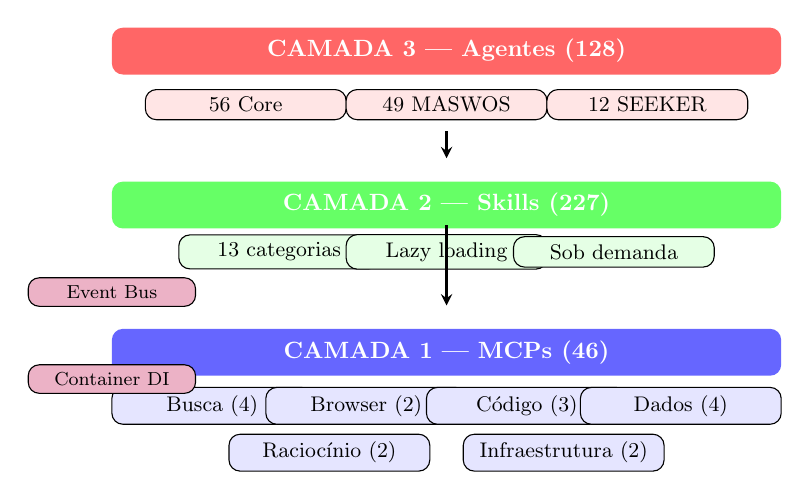
\begin{tikzpicture}[scale=0.85, every node/.style={scale=0.85},
  layer/.style={rectangle, rounded corners, minimum width=10cm, minimum height=0.7cm,
                font=\bfseries, text=white},
  comp/.style={rectangle, draw, rounded corners, minimum width=3cm, minimum height=0.45cm,
               font=\small},
  arrow/.style={->, thick, >=stealth}
]
  % Camada 3
  \node[layer, fill=red!60] at (0,3.5) {CAMADA 3 --- Agentes (128)};
  \node[comp, fill=red!10] at (-3,2.7) {56 Core};
  \node[comp, fill=red!10] at (0,2.7) {49 MASWOS};
  \node[comp, fill=red!10] at (3,2.7) {12 SEEKER};

  % Camada 2
  \node[layer, fill=green!60] at (0,1.2) {CAMADA 2 --- Skills (227)};
  \node[comp, fill=green!10] at (-2.5,0.5) {13 categorias};
  \node[comp, fill=green!10] at (0,0.5) {Lazy loading};
  \node[comp, fill=green!10] at (2.5,0.5) {Sob demanda};

  % Camada 1
  \node[layer, fill=blue!60] at (0,-1) {CAMADA 1 --- MCPs (46)};
  \node[comp, fill=blue!10] at (-3.5,-1.8) {Busca (4)};
  \node[comp, fill=blue!10] at (-1.2,-1.8) {Browser (2)};
  \node[comp, fill=blue!10] at (1.2,-1.8) {Código (3)};
  \node[comp, fill=blue!10] at (3.5,-1.8) {Dados (4)};
  \node[comp, fill=blue!10] at (-1.75,-2.5) {Raciocínio (2)};
  \node[comp, fill=blue!10] at (1.75,-2.5) {Infraestrutura (2)};

  % Setas
  \draw[arrow] (0,2.3) -- (0,1.9);
  \draw[arrow] (0,0.9) -- (0,-0.3);

  % Barramento
  \node[draw, fill=purple!30, rounded corners, minimum width=2.5cm, minimum height=0.4cm,
        font=\footnotesize] at (-5,-0.1) {Event Bus};
  \node[draw, fill=purple!30, rounded corners, minimum width=2.5cm, minimum height=0.4cm,
        font=\footnotesize] at (-5,-1.4) {Container DI};
\end{tikzpicture}
\end{figure}

% =============================================================================
%  SEÇÃO 3: OS 6 SCANNERS EPISTEMOLÓGICOS
% =============================================================================
\section*{Os 6 Scanners Epistemológicos}

O pipeline de scanners do \opencodeeco{} forma um sistema completo de
diagnóstico e planejamento evolutivo:

\begin{table}[htb]
\centering
\caption{Os 6 scanners do pipeline epistemológico}
\label{tab:cheatsheet-scanners}
\small
    \resizebox{\textwidth}{!}{
\begin{tabular}{lllll}
\toprule
\textbf{Scanner} & \textbf{SPEC} & \textbf{Pergunta} & \textbf{Entrada} & \textbf{Saída} \\
\midrule
Potentiality    & 043 & O que existe?      & workspace        & DNA estrutural \\
Noological      & 028 & O que não existe?  & DNA + corpus     & Gaps e zonas \\
Teleológico     & 029 & O que deveria existir? & Objetivos + gaps & Lacunas teleológicas \\
Evolutivo       & 030 & Qual o melhor caminho? & Lacunas + analogias & Roadmap \\
Refinement      & 031 & Como refinar?      & Roadmap          & Gaps refinados \\
MCSP            & 032 & Conjunto mínimo?   & Gaps refinados   & Capacidades mínimas \\
\bottomrule
\end{tabular}
    }
\end{table}

\noindent O \textbf{Capability Composer} (SPEC-033/035) recebe as saídas de
todos os scanners e decompõe capacidades em insumos cognitivos atômicos.
O \textbf{Potentiality Scanner} (SPEC-043) alimenta o pipeline com o
diagnóstico inicial do estado atual do ecossistema.

% =============================================================================
%  SEÇÃO 4: MAPA DE DEPENDÊNCIAS ENTRE SPECS
% =============================================================================
\section*{Mapa de Dependências entre SPECs}

O diagrama a seguir ilustra as relações de dependência entre as 13 SPECs
do \opencodeeco{}:

\begin{figure}[htb]
\centering
\caption{Dependências entre SPECs}
\label{fig:cheatsheet-specs}
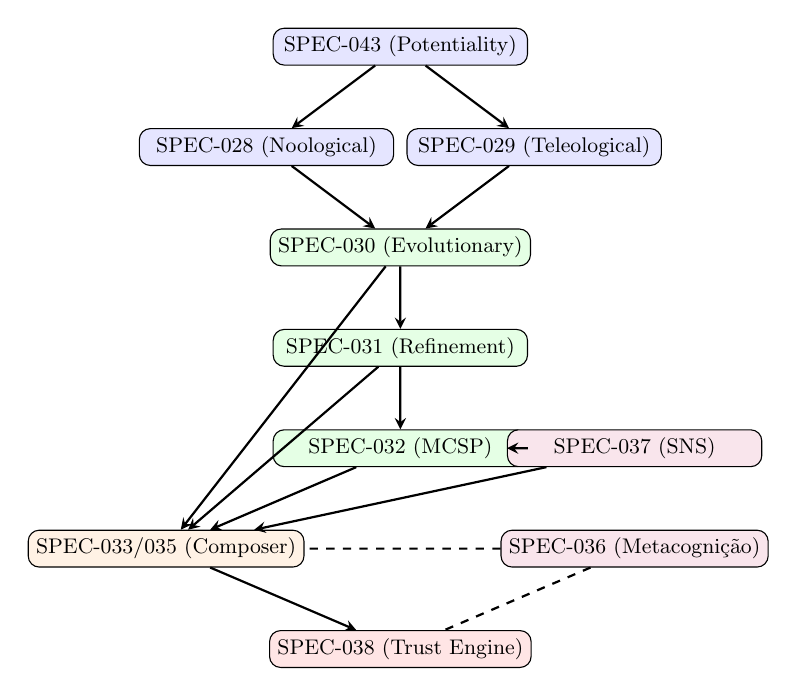
\begin{tikzpicture}[scale=0.85, every node/.style={scale=0.85},
  spec/.style={rectangle, draw, rounded corners, minimum width=3.8cm, minimum height=0.5cm,
               font=\small},
  arrow/.style={->, thick, >=stealth},
  super/.style={=>, thick, >=stealth, dashed}
]
  \node[spec, fill=blue!10] (P) at (0,3.5) {SPEC-043 (Potentiality)};
  \node[spec, fill=blue!10] (N) at (-2,2) {SPEC-028 (Noological)};
  \node[spec, fill=blue!10] (T) at (2,2) {SPEC-029 (Teleological)};
  \node[spec, fill=green!10] (E) at (0,0.5) {SPEC-030 (Evolutionary)};
  \node[spec, fill=green!10] (R) at (0,-1) {SPEC-031 (Refinement)};
  \node[spec, fill=green!10] (M) at (0,-2.5) {SPEC-032 (MCSP)};
  \node[spec, fill=orange!10] (C) at (-3.5,-4) {SPEC-033/035 (Composer)};
  \node[spec, fill=purple!10] (S) at (3.5,-4) {SPEC-036 (Metacognição)};
  \node[spec, fill=purple!10] (Q) at (3.5,-2.5) {SPEC-037 (SNS)};
  \node[spec, fill=red!10] (X) at (0,-5.5) {SPEC-038 (Trust Engine)};

  \draw[arrow] (P) -- (N);
  \draw[arrow] (P) -- (T);
  \draw[arrow] (N) -- (E);
  \draw[arrow] (T) -- (E);
  \draw[arrow] (E) -- (R);
  \draw[arrow] (R) -- (M);
  \draw[arrow] (M) -- (C);
  \draw[arrow] (R) -- (C);
  \draw[arrow] (E) -- (C);
  \draw[super] (S) -- (C);
  \draw[super] (S) -- (X);
  \draw[arrow] (Q) -- (C);
  \draw[arrow] (M) -- (Q);
  \draw[arrow] (C) -- (X);
\end{tikzpicture}
\end{figure}

\noindent Setas sólidas indicam fluxo de dados; setas tracejadas indicam
supervisão. A SPEC-036 (Metacognição) supervisiona todo o pipeline. A
SPEC-038 (Trust Engine) é a camada final de segurança sobre todas as
demais.

% =============================================================================
%  SEÇÃO 5: LINHA DO TEMPO DOS CICLOS EVOLUTIVOS
% =============================================================================
\section*{Linha do Tempo Evolutiva (R1-R23)}

A Tabela~\ref{tab:cheatsheet-ciclos} apresenta a trajetória evolutiva
completa do \opencodeeco{}, do R1 ao R23.

\begin{table}[htb]
\centering
\caption{Ciclos evolutivos R1-R23 (versão condensada)}
\label{tab:cheatsheet-ciclos}
\small
    \resizebox{\textwidth}{!}{
\begin{tabular}{cllcc}
\toprule
\textbf{Release} & \textbf{Período} & \textbf{Capacidade Gerada} & \textbf{CTs} & \textbf{Score} \\
\midrule
R1  & 2024.1 & Validação quantitativa World Bank        & --- & 85 \\
R2  & 2024.1 & Pipeline de artigos acadêmicos           & --- & 90 \\
R3  & 2024.2 & Citações TSAC, Sci-Hub, validação        & --- & 92 \\
R4  & 2024.2 & Ciclo de correção iterativa v2.0         & --- & 95 \\
R5  & 2024.3 & Corretor linguístico CJK                 & --- & 98 \\
R6  & 2024.3 & Editais-br v2.0, 4 categorias            & --- & 92 \\
R7  & 2024.4 & Editais-br v7.1, cache versionado        & --- & 94 \\
R8  & 2024.4 & SDD+TDD acadêmico, simulação de banca    & 9   & 94 \\
R9  & 2025.1 & AutoEvolve LaTeX, framework docs         & 16  & 96 \\
R10 & 2025.1 & Menu adaptativo, plugin system           & --- & 96 \\
R11 & 2025.1 & CORA-Eval Benchmark (150 tarefas)        & --- & 97 \\
R12 & 2025.2 & Science Skills Core, MCP Expansion       & --- & 98 \\
R13 & 2025.2 & Reasoning Engines (Z3, SymPy, Kanren...) & --- & 96 \\
R14 & 2025.2 & Ampliação: 227 skills, 128 agentes       & --- & 97 \\
R15 & 2025.3 & Agentes acadêmicos, pipeline Qualis A1   & --- & 98 \\
R16 & 2025.3 & Autoevolve + Manus Evolve + Sync         & --- & 98 \\
R17 & 2025.3 & Gartner Hype Cycle 2026, 3 gaps          & 24  & 99 \\
R18 & 2025.4 & Token Economy Core (SPEC-022)            & 9   & 99 \\
R18b& 2025.4 & Agent Economics + Audit (SPEC-023/024)    & 10  & 99 \\
R19 & 2025.4 & MCSP + 5 scanners (SPEC-028 a 032)       & 76  & 99 \\
R20 & 2026.1 & Composição Unitária do Conhecimento       & 19  & 100 \\
R21 & 2026.1 & Metacognição + Self-Evolution (SPEC-036) & 8   & 100 \\
R22 & 2026.1 & SNS + N3 completo (SPEC-037)             & 22  & 100 \\
R23 & 2026.1 & Trust Engine + N3.5 (SPEC-038)           & 8   & 100 \\
\midrule
\multicolumn{3}{l}{\textbf{Total}} & \textbf{312} & \textbf{100\%} \\
\bottomrule
\end{tabular}
    }
\end{table}

\noindent \textbf{Legenda:} CTs = casos de teste; Score = avaliação
AUTO\_SCORE\_QUALIS (0--100). Período aproximado (ano.trimestre).
Scores $\geq$ 95 indicam padrão Qualis A1.

% =============================================================================
%  SEÇÃO 6: GLOSSÁRIO DE TERMOS TÉCNICOS ESTENDIDO
% =============================================================================
\section*{Glossário Técnico Rápido}

\begin{description}

\item[MCP] \emph{Model Context Protocol} --- protocolo padrão para comunicação
entre modelos de IA e ferramentas externas. 46 servidores integrados.

\item[Skill] Habilidade especializada do ecossistema, contendo instruções
para a IA executar uma tarefa específica. 227 skills em 13 categorias.

\item[Agente] Orquestrador inteligente que coordena MCPs e skills para
atingir um objetivo. 128 agentes especializados.

\item[Barramento (Event Bus)] Mecanismo de comunicação assíncrona
publish-subscribe entre componentes do ecossistema.

\item[Scanner] Módulo de diagnóstico que analisa um aspecto específico do
ecossistema (ex.: Noological, Teleológico, Evolutivo).

\item[SPEC] \emph{Specification} --- documento formal que define requisitos,
critérios de aceitação e arquitetura de um componente. 13 SPECs.

\item[ADR] \emph{Architecture Decision Record} --- registro de decisão
arquitetural com rationale, contexto e consequências. 10 ADRs.

\item[CT] \emph{Case Test} --- caso de teste unitário ou de integração.
312 CTs com 100\% de aprovação contínua.

\item[TDD] \emph{Test-Driven Development} --- metodologia em que os testes
são escritos antes do código de produção.

\item[SDD] \emph{Spec-Driven Development} --- metodologia em que a
especificação formal precede a implementação e os testes.

\item[Qualis A1] Classificação máxima no sistema Qualis da CAPES para
periódicos e produção científica.

\item[TSAC] \emph{Text Style Anti-Cloning} --- técnica de detecção e
prevenção de textos similares a saídas de IA, com 87 palavras proibidas.

\item[MCSP] \emph{Minimum Capability Set Problem} --- problema de seleção
do conjunto mínimo de capacidades para cobrir funcionalidades requeridas.

\item[N0 a N4] Níveis de auto-consciência artificial: N0 (inconsciente),
N1 (reativo), N2 (automatizado), N3 (metacognitivo), N3.5 (com Behavioral
Gate preventivo), N4 (autoconsciente pleno --- teórico).

\item[Trust Engine] Sistema integrado de TrustScorer, Behavioral Gate,
NaturalForgetting e OutcomeTracker (SPEC-038).

\item[Behavioral Gate] Componente do Trust Engine que classifica ações em
safe, moderate, risky ou blocked antes da execução.

\item[Token Economy] Sistema de incentivos econômicos baseado em tokens
para recompensar contribuições ao ecossistema (SPEC-022 a 024).

\item[Fee Market] Mercado dinâmico de taxas para uso de recursos do
ecossistema, com preços ajustados por oferta e demanda.

\item[Staking] Mecanismo de bloqueio de tokens por 7 dias para participar
da governança do ecossistema.

\item[Slashing] Penalidade de redução de stake por comportamento malicioso
ou negligente.

\item[MASWOS] \emph{Multi-Agent System for Writing and Orienting Scientific}
--- sistema multiagente com 49 agentes para produção acadêmica.

\item[SEEKER] Sistema de pesquisa com 10 agentes inteligentes e motor de
árvore de argumentos para fundamentação acadêmica.

\item[Reversa] Conjunto de 18 agentes especializados em engenharia reversa,
refatoração e análise de código legado.

\item[Manus Evolve] Motor de evolução autônoma que gerencia o ciclo
PLAN$\to$ACT$\to$REFLECT$\to$EXTRACT$\to$EVOLVE.

\item[Corretor CJK] Script Python (\codigo{ptbr\_corrector.py}) que detecta
e remove caracteres CJK, garantindo saída em português brasileiro formal.

\item[Nexus] Camada de orquestração multiagente com 488 arquivos, 120+
barreiras de sincronização e 212+ tipos de raciocínio.

\item[MiroFish] Conjunto de 11 ferramentas de modelagem multiagente
(OASIS, Forum, Config, Graph, Report, Nash, Stats\dots).

\item[BettaFish] Conjunto de ferramentas de análise acadêmica complementar
ao MiroFish (QualisA1Auditor, SensitivityAnalyzer, IMRADFormatter\dots).

\item[Potentiality Scanner] Scanner que mapeia o estado atual do
ecossistema, identificando capacidades existentes e emergentes (SPEC-043).

\item[Composição Unitária] Metodologia de decomposição de capacidades em
6 tipos de insumos cognitivos atômicos (SPEC-033/035).

\item[SNS] \emph{Structural Noise Scanner} --- compressor estrutural com
preservação funcional para processamento de grandes textos (SPEC-037).

\end{description}
